\section{Marco Aplicativo}

\subsection{Método de Desarrollo}

Para llevar a cabo el cumplimiento de los objetivos, es necesario definir un esquema o metodología de trabajo que permita la elaboración de un conjunto de
lineamientos de manera estructurada y organizada.
Por lo tanto, se hace uso de el método de Desarrollo Rápido de Aplicaciones (RAD), el cual permite la iteración rápida y continua de pequeños objetivos para alcanzar la meta final.

RAD es un proceso de desarrollo de software que
integra un conjunto de técnicas, lineamientos y herramientas que permiten llevar a cabo, en
cortos periodos de tiempo, la implementación de funcionalidades en un sistema, de tal manera que
satisfacen las necesidades del cliente \cite{23}.
Siguiendo esta metodología, el software evoluciona y crece durante el proceso de desarrollo en base a la retro alimentación que se tiene con el cliente.
De esta manera, se realizan múltiples entregas de una tarea que
contiene las nuevas funcionalidades esperadas.
Cada una de estas tareas cuenta con instrumento de documentación al cuál llamaremos historias.
Estas historias describen los detalles técnicos e categorizan las tareas en subgrupos.

Por medio de RAD, fue posible la implementación de la solución al problema previamente planteado a través del desarrollo de múltiples componentes relacionados entre si, para
brindar un servicio web como un API.
La figura \ref{fig:diagram_general} muestra la arquitectura general del servicio web, y como interactuá con las aplicaciones clientes que lo consumen.

\begin{figure}[H]
	\centering
		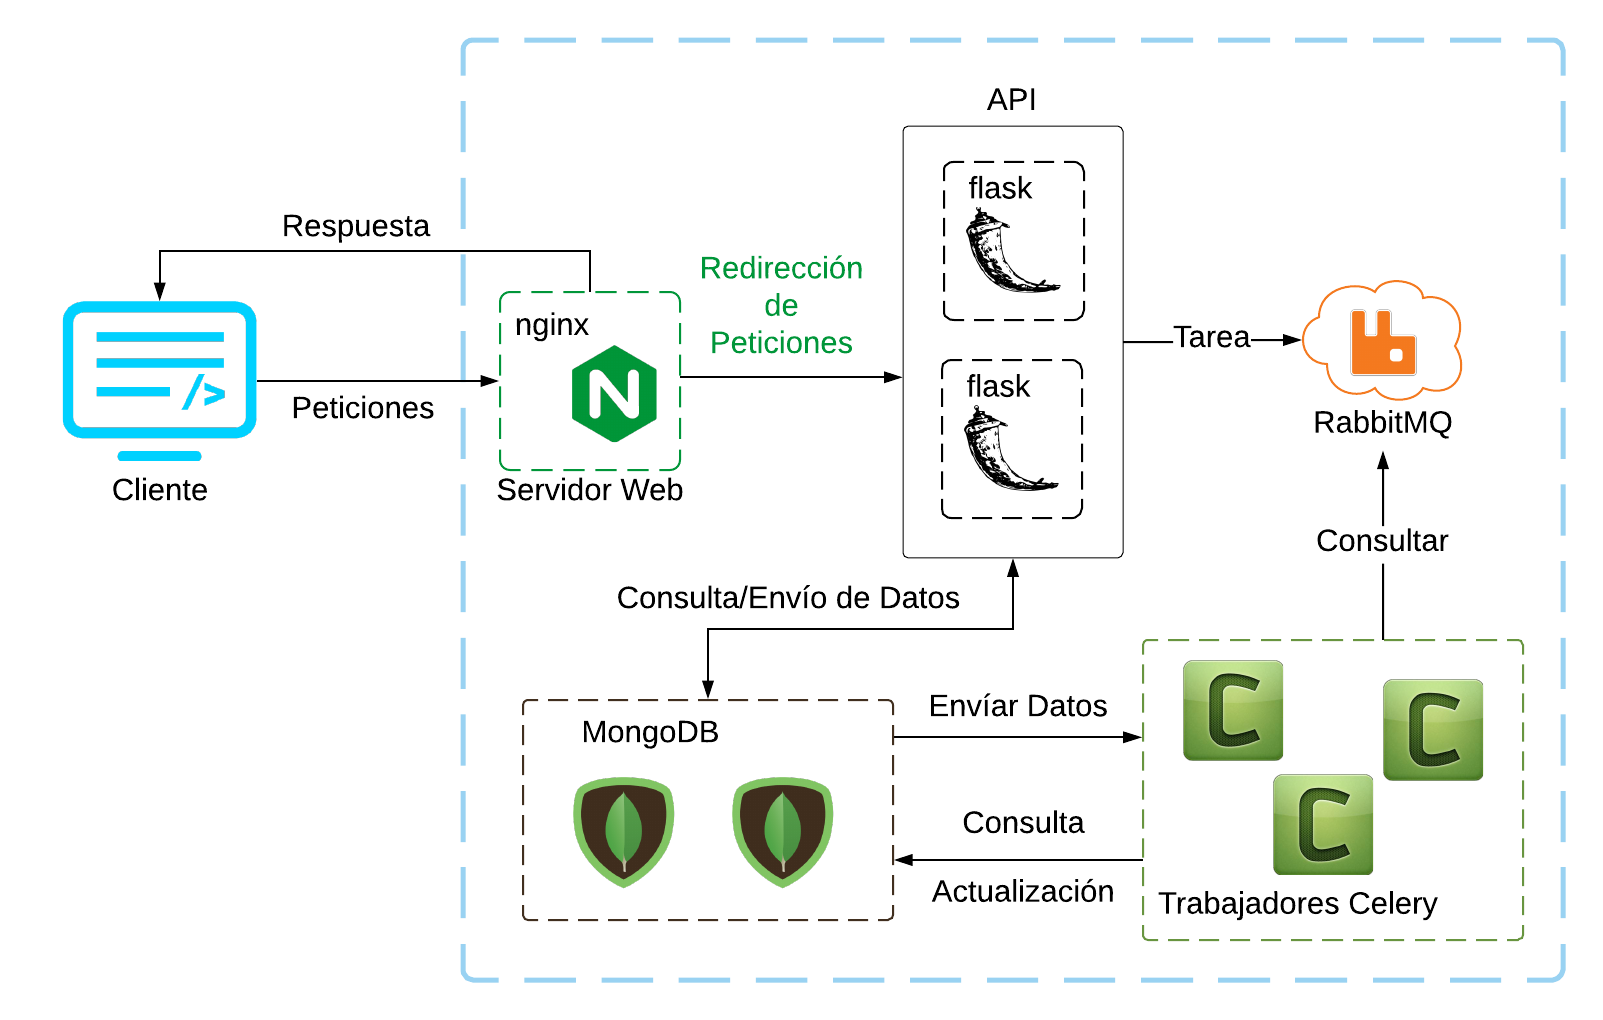
\includegraphics[width=1\textwidth]{figures/diagram_general}
	\caption{Arquitectura general de la aplicación}
	\label{fig:diagram_general}
\end{figure}

Los componentes que conforman este servicio son los siguientes

\begin{itemize}

\item Un servidor web (Nginx) que atiende, en primera instancia, las peticiones de las aplicaciones clientes y balancea la carga entre múltiple nodos que almacenan el API.

\item Una o más aplicaciones Flask, almacenadas en máquinas separadas, que ejecutan el API e inician las tareas de consulta y extracción de revisiones.

\item Un servicio de mensajería (RabbitMQ) que recibe las tareas iniciadas por el API
y las encola para su posterior ejecución.

\item Uno o más nodos que ejecutan un proceso trabajador de Celery para la ejecución de las tareas almacenadas en RabbitMQ.
Estos nodos mantienen una comunicación con RabbitMQ para actualizar el estado y progreso de las tareas.

\item Y, por último, un componente de almacenamiento de artículos wiki y sus revisiones. Para ello se hace uso de MongoDB y está implementado como un cluster de base de datos distribuidos
entre múltiples máquinas conectadas entre sí que permiten la fragmentación de los datos.

\end{itemize}

\subsection{Servidor Web}

El servidor web que atiende las solicitudes en primera instancia es Nginx,
el cual funciona como un intermediario entre el cliente y el API que responde dicha solicitud.
Nginx permite balancear la carga de trabajo entre múltiples servidores que contienen la aplicación mediante el algoritmo de round robin,
de tal forma que cada servidor es utilizado de forma equitativa, tal como se muestra en la figura \ref{fig:round_robin}.

\begin{figure}[H]
	\centering
		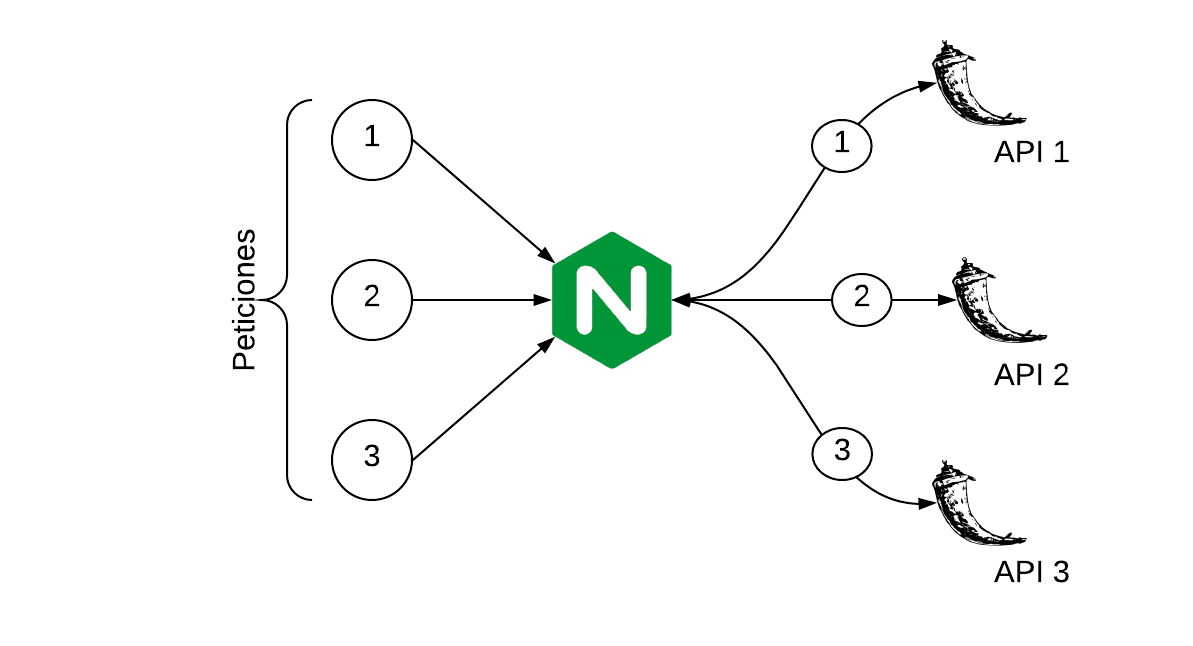
\includegraphics[width=0.9\textwidth]{figures/round_robin}
	\caption{Algoritmo de distribución de peticiones de Nginx basado en método de Round Robin.}
	\label{fig:round_robin}
\end{figure}

Una vez la petición ha sido reasignada, es atendida por medio del servidor web UWSGI, y en conjunto
con Flask y el resto de las tecnologías incluidas en el API, genera una respuesta de vuelta al cliente.

\subsection{API}

El API diseñado para realizar las labores de extracción y consulta de las revisiones, hace uso del lenguaje de programación Python \texttt{2.7.10} y el uso del framework Flask \texttt{v0.12}.
Ambas tecnologías permiten la asignación de rutas específicas para cada módulo
y la atención de peticiones.

La interacción entre el servicio y una aplicación cliente puede ser apreciada en la figura \ref{fig:diagram_api_1}.

\begin{figure}[H]
	\centering
		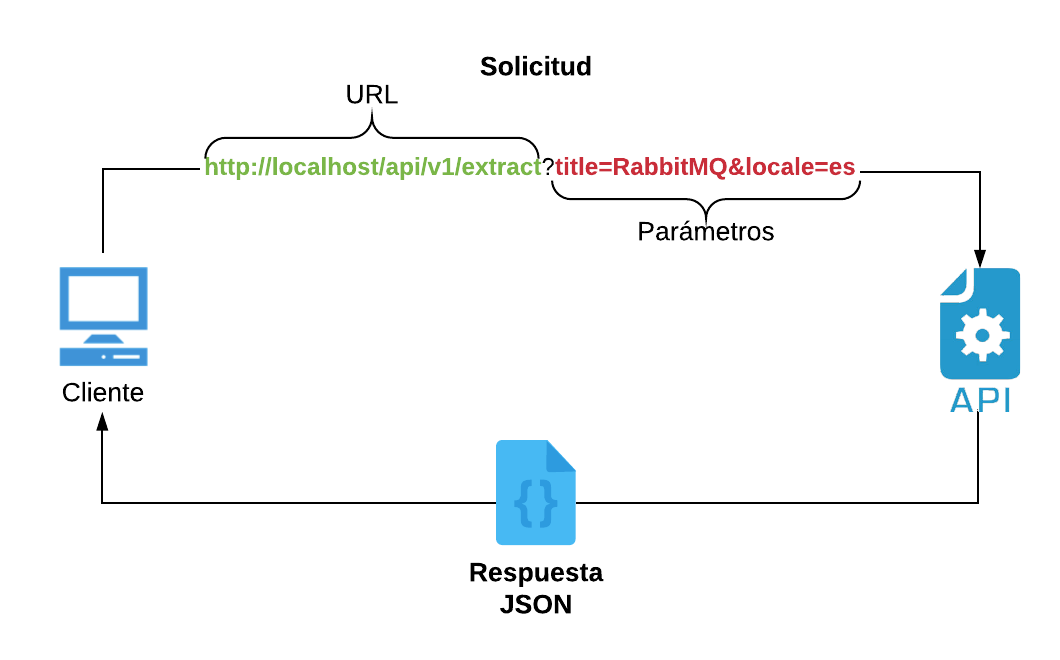
\includegraphics[width=1\textwidth]{figures/diagram_api_1}
	\caption{Interacción entre una aplicación cliente y el API}
	\label{fig:diagram_api_1}
\end{figure}

Esta interacción se basa en la petición de un recurso o de un proceso, por parte de una aplicación cliente, a una ruta del servidor web (endpoint).
Cada petición puede incluir parámetros opcionales para la paginación, filtrado de resultados, como por ejemplo, el idioma del artículo a extraer.

Las rutas de acceso que ofrece el API son las siguientes:

\begin{itemize}
	\item \texttt{/api/v1/articles}. Listado de todos los artículos extraídos.
	\item \texttt{/api/v1/revisions}. Listado de las revisiones de los artículos extraídos.
	\item \texttt{/api/v1/extract}. Extracción de revisiones de artículos wiki.
	\item \texttt{/api/v1/avg}. Cálculo del promedio de revisiones de un artículo por rango fechas.
	\item \texttt{/api/v1/count}. Cálculo de número de revisiones de un artículo por fecha.
	\item \texttt{/api/v1/mode}. Cálculo de las revisiones mas extraídas por rango de fecha.
	\item \texttt{/api/v1/status}. Indica el estado del proceso de extracción.
	\item \texttt{/api/v1/query}. Permite la ejecución de consultas personalizadas a la base de datos.
\end{itemize}

\subsubsection{Extracción de Historiales}

Para la extracción de historiales se hace uso de la ruta de acceso \texttt{/api/v1/extract}, la cual
tiene como parámetros:
\texttt{title}, que se refiere al título del del artículo; \texttt{url}, representa la ruta completa de un artículo, por ejemplo:
\texttt{https://en.wikipedia.org/wiki/The\_Lord\_of\_the\_Rings}; y por último, \texttt{locale}, el cual índica el idioma del artículo y
es completamente opcional, puesto que el sistema asume el inglés como lenguaje por defecto o lo extrae del parámetro
\texttt{url}.
Es necesario proporcionar el parámetro \texttt{url} o \texttt{title} de forma obligatoria para poder llevar a cabo la extracción.

En la figura \ref{fig:extract_url_format} se puede apreciar dos ejemplos del uso de los parámetros \texttt{url}, \texttt{title} y \texttt{locale}:

\begin{figure}[H]
	\centering
		
\includegraphics[width=1\textwidth]{figures/extract_url_format}
	\caption{Parámetros para la extracción de historiales}
	\label{fig:extract_url_format}
\end{figure}

La ejecución de esta tarea se lleva a cabo por medio de Celery y RabbitMQ.
Con estas tecnologías, múltiples computadores ejecutan un proceso de Celery, los
cuales están conectados entre si gracias a RabbitMQ, escuchando constantemente los mensajes entrantes de este servicio.
Una vez recibida la petición por el API, se genera una tarea de extracción por medio de Celery, la cual tiene un identificador único.
Esta tarea es encolada en una lista de
espera que es atendida por uno de los trabajadores conectados a RabbitMQ y es ejecutada en segundo plano.
Posteriormente, el API crea una respuesta a la petición generando una ruta para consultar el progreso
del proceso de extracción, la cual luce como se muestra en la figura \ref{fig:extract_response}:

\begin{figure}[H]
	\centering
		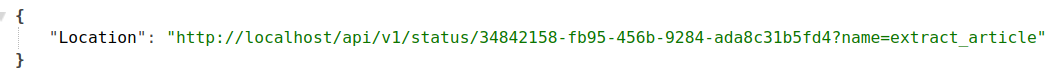
\includegraphics[width=1\textwidth]{figures/extract_response}
	\caption{Respuesta a una petición de extracción de historiales de un artículo}
	\label{fig:extract_response}
\end{figure}

Durante el proceso de extracción, se realizan peticiones hacia el API de Wikipedia.
Se toma como URL por defecto la dirección https://en.wikipedia.org/w/api.php, en conjunto con diversos parámetros, tales como:

\begin{itemize}
	\item \textbf{action}: tipo de petición que se realiza sobre este API, en este caso se hace uso del valor \texttt{query} para indicar que solo se realizará una consulta.

	\item \textbf{format}: formato de la respuesta obtenida, la cual puede ser XML o JSON.

	\item \textbf{props}: la propiedad del artículo al cual se desea consultar, en este caso se usa el valor \texttt{revisions} para poder extraer el historial de modificaciones del mismo.

	\item \textbf{rvprop}: atributos de la propiedad extraída, los incluidos para esta extracción son los siguientes: ids, flags, timestamp, user, userid, size, sha1, contentmodel, comment, parsedcomment, content, tags.

	\item \textbf{rvlimit}: permite la paginación de los resultados e indica la cantidad de resultados que se quieren obtener por página.

	\item \textbf{newer}: permite ordenar las revisiones de forma ascendente o descendiente acorde a la fecha de creación. Se ordenan de forma descendente usando el valor \texttt{newer}, de esta manera es más rápido extraer las revisiones mas recientes.
\end{itemize}

Justo antes de enviar la solicitud al API de wikipedia, se verifica que el artículo a consultar ya esté almacenado en la base de datos, en caso de no estarlo, se almacena indicando la fecha de extracción.
Posteriormente, se extraen sus revisiones, y puesto que la respuesta del API coloca las revisiones mas recientes al principio, el extractor culmina su ejecución una vez determina que alcanzó una revisión que ya ha sido almacenada.
Al almacenar las revisiones en la base de datos, se actualiza el documento del artículo con la fecha de la última extracción y el identificador de la revisión extraída, y por último, se actualiza el progreso de la tarea.
Por cada página de revision extraída, el sistema espera un segundo para ejecutar la siguiente llamada al API, de esta manera se respetan los líneamientos recomendados por Mediawiki para la consulta de los datos y evitar
la sobrecarga de su servicio. 

En la figura \ref{fig:response_status} se puede apreciar un ejemplo de la consulta del progreso de las tareas:

\begin{figure}[H]
	\centering
		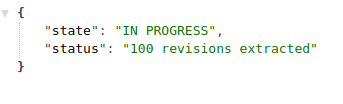
\includegraphics[width=0.8\textwidth]{figures/response_status}
	\caption{Respuesta a una petición para consultar de progreso de una tarea de extracción}
	\label{fig:response_status}
\end{figure}

La tabla \ref{tab:extract} muestra la historia asociada a la extracción de revisiones.


\renewcommand{\arraystretch}{1.5}
\begin{table}[H]
	\begin{center}
		\begin{tabular}{|l|r|}
			\hline
			\multicolumn{2}{|r|}{\textbf{Historia}} \\
			\hline
			\textbf{Desarrollador} & Marvin Bernal\\
			\hline
			\textbf{Nombre} & Extracción de revisiones por API\\
			\hline
			\textbf{Sección} & Extracción\\
			\hline
			\textbf{Descripción} & \parbox[t]{3in}{Extracción de todas las revisiones de un artículo
				wiki dado su título a través del API que ofrece mediawiki \par
				Se realiza una petición sobre el URL
				\texttt{https://en.wikipedia.org/w/api.php} y se agregan parámetros
				extra, incluyendo el título del artículo, para obtener todos los
				metadatos posibles de una revisión.
				\par
				Cada petición al API obtiene un máximo de 50 revisiones se llevan
				a cabo con una diferencia de 2 segundos.}\\
			\hline
			\textbf{Observaciones} & \parbox[t]{3in}{Se extraen los siguientes datos: id de la revisión, tipo de revisión,
			fecha, nombre de usuario, id de usuario, tamaño, comentarios,
			contenido y etiquetas}\\
			\hline
		\end{tabular}
		\caption{Extracción de Revisiones}
		\label{tab:extract_revisions}
	\end{center}
\end{table}


\subsubsection{Consultas}

El API consta de métodos de acceso para consultar las revisiones extraídas y
los artículos asociados a través de las rutas \texttt{/api/v1/revisions} y \texttt{/api/v1/articles} respectivamente.

En estas rutas de consulta es posible hacer uso de diversos parámetros de búsqueda,
entre ellas están: los parámetros de paginación \texttt{page} y \texttt{page\_size},
y los parámetros de búsqueda que corresponden a los atributos del artículo,
tales como: \texttt{title}, \texttt{first\_extraction\_date}, \texttt{last\_extraction\_date}, \texttt{last\_revision\_extracted} y \texttt{locale}.
Adicionalmente, existe el parámetro \texttt{sort}, que permite ordenar los resultados a través del valor de un atributo de la colección a consultar, ejemplo, por la fecha de extracción de un artículo.

La ruta \texttt{articles} tiene como finalidad mostrar la información pertinente a los artículos que han sido extraídos a través del API, para lo cual se realiza una consulta a la colección \texttt{articles} almacenada en la base de datos. Un ejemplo de la respuesta obtenida por esta ruta puede ser apreciada en la figura \ref{fig:response_articles}.

\begin{figure}[H]
	\centering
		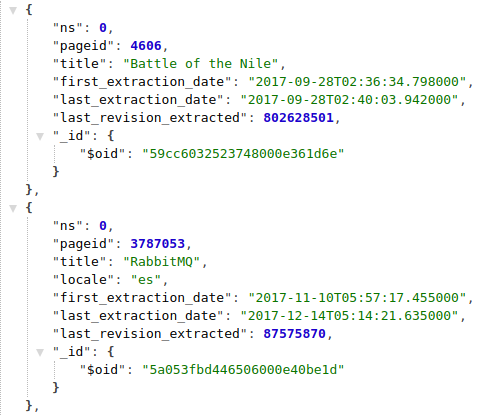
\includegraphics[width=0.8\textwidth]{figures/response_articles}
	\caption{Respuesta a una petición de consulta de artículos}
	\label{fig:response_articles}
\end{figure}

Por su parte, la ruta \texttt{revisions} permite consultar el contenido y los datos pertinentes a las revisiones que han sido extraídas.
En la figura \ref{fig:response_revisions} se puede apreciar una respuesta del servidor a la consulta de revisiones.

\begin{figure}[H]
	\centering
		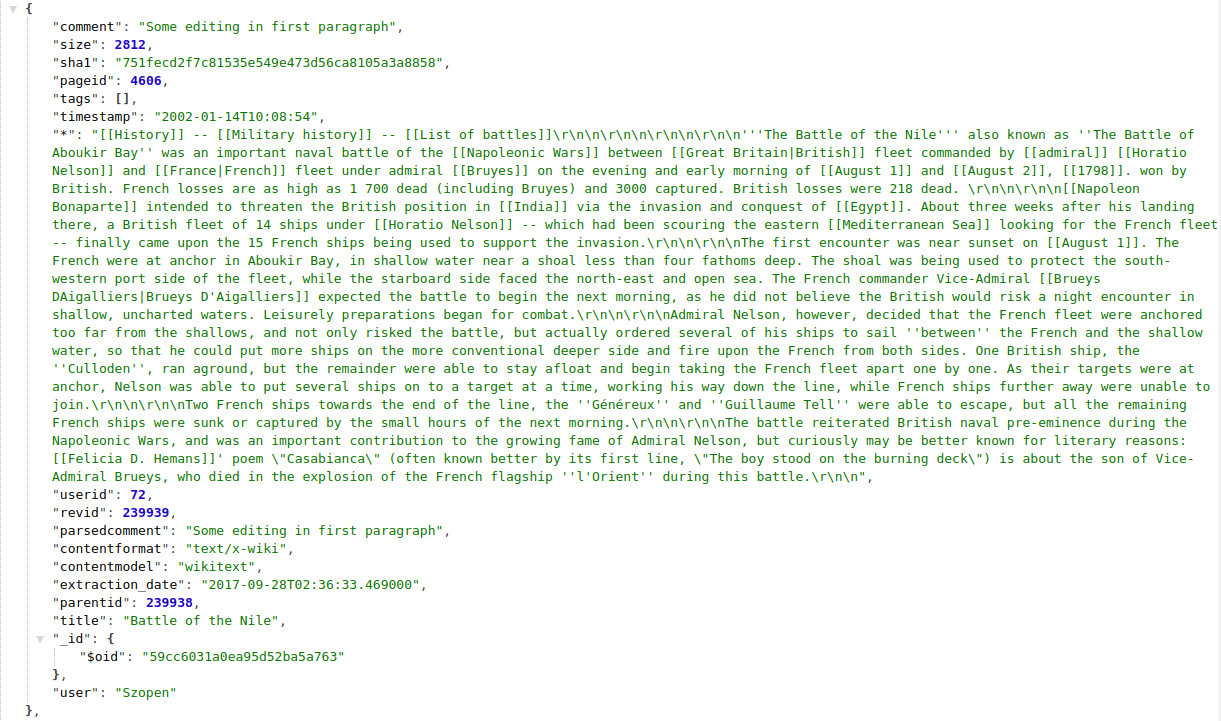
\includegraphics[width=1\textwidth]{figures/response_revisions}
	\caption{Respuesta a una petición de consulta de revisiones}
	\label{fig:response_revisions}
\end{figure}

Adicionalmente, existen mas rutas de acceso al API para la consulta de diversas métricas predefinidas, tales como: promedio, conteo de revisiones y moda.

Durante el cálculo de estas métricas se toman como parámetros múltiples atributos, tales como: el título del artículo o la fecha de extracción.
Dichos atributos son usados para reducir o filtrar las revisiones que se van a consultar en el cálculo de  métricas.

Antes que los parámetros de búsqueda sean utilizados, pasan por un proceso de aceptación, en donde sólo son tomados en cuenta aquellos parámetros incluidos en una lista denominada \textit{Lista Blanca}, mientras que el resto son ignorados.

Posteriormente, se genera una tarea que será procesada en segundo plano por medio de Celery, con el tipo de consulta a realizar y los parámetros de búsqueda.

El formato de algunos atributos utilizados en el proceso de búsqueda de revisiones o artículos, tales como, fecha de extracción y tamaño de la revisión, es alterado para facilitar la consulta de revisiones por un rango o intervalo determinado.
Para los atributos que representan una fecha, se condiciona la búsqueda en base a una fecha única o un intervalo de fechas por medio de los parámetros recibidos en la petición.
Para atributos que representan el tamaño se ejecuta un proceso similar, donde se considera un segundo argumento opcional que indica el intervalo a evaluar para condicinar la consulta.

En la tabla \ref{tab:count} se puede apreciar, con detalle, y por medio de su historia, las condiciones de búsqueda aceptadas por dicha consulta.


\renewcommand{\arraystretch}{1.5}
\begin{table}[H]
	\begin{center}
		\begin{tabular}{|l|r|}
			\hline
			\multicolumn{2}{|r|}{\textbf{Historia}} \\
			\hline
			\textbf{Desarrollador} & Marvin Bernal\\
			\hline
			\textbf{Nombre} & Endpoint para el cálculo de la cantidad de revisiones\\
			\hline
			\textbf{Sección} & Consulta\\
			\hline
			\textbf{Descripción} & \parbox[t]{3in}{Parte del API de la solución distribuida donde el endpoint \texttt{/count}
			recibe como parámetros los atributos para restringir o filtrar el
			rango a tomar en cuenta como resultado. Los argumentos
			disponibles hasta el momento son:\par
				\begin{itemize}

					\item title: título del artículo extraído.
					\item pageid: id del artículo extraído.
					\item user: nombre del usuario que realiza la revisiones.
					\item userid: id del usuario que realiza la revisiones.
					\item tag: una etiqueta determinada que contenga las
					revisiones.
					\item size: el tamaño de la revisión realizada.
					\item sizematch: valor que acompaña a \texttt{size}. Si el valor es
					positivo, se filtrarán todas las revisiones de mayor
					tamaño que el valor de \texttt{size}. Si es negativo, se filtrarán
					todas las revisiones de menor tamaño que el valor de
					\texttt{size}. Si el valor es 0 o no se encuentra en los parámetros
					de la solicitud, se filtrarán todas las revisiones cuyo
					tamaño sea exactamente el valor de \texttt{size}.
					\item date: la fecha exacta en que fueron realizadas las
					revisiones. El formato de fecha utilizado es: \texttt{YYYY-MM-DD}.
					\item datestart: la fecha inicial a partir de la cual fueron
					realizadas las revisiones en un intervalo de tiempo. El
					formato de fecha utilizado es: \texttt{YYYY-MM-DD}. En caso de
					que no exista el parámetro \texttt{dateend} en la solicitud, la fecha final del intervalo será la fecha actual.
					\item dateend: la fecha final hasta la cual fueron realizadas las
					revisiones en un intervalo de tiempo. El formato de
					fecha utilizado es: \texttt{YYYY-MM-DD}. En caso de que no
					exista el parámetro \texttt{datestart} en la solicitud, la fecha
					inicial del intervalo será la fecha de la primera revisión
					del artículo.
				\end{itemize}
				\\
			\hline
			\textbf{Observaciones} & \parbox[t]{3in}{Primero se realiza una comprobación de los parámetros de la
solicitud contra una lista blanca con los parámetros permitidos.
Luego, con los parámetros resultantes, se realiza el
procesamiento a través de una tarea asignada, para luego
devolver el resultado.}\\
			\hline
		\end{tabular}
		\caption{Extracción de Revisiones}
		\label{tab:extract_revisions}
	\end{center}
\end{table}


La consulta del promedio revisiones se calcula haciendo uso de intervalos de tiempos (en este caso, días), determinados por el usuario en la petición al servicio.
En la tabla \ref{tab:average} se presentan con mayor con detalle, por medio de su historia, los filtros aceptados, así como los argumentos obligatorios de la consulta.

\begin{longtable}{|l|m{4in}|}

\hline
\multicolumn{2}{|r|}{\textbf{Historia}} \\
\hline
\endfirsthead

\multicolumn{2}{c}%
{{\bfseries \tablename\ \thetable{} -- continuación de la página anterior}} \\
\hline \multicolumn{2}{|r|}{\textbf{Historia}} \\ \hline
\endhead

\textbf{Desarrollador} & Marvin Bernal \\
\hline
\textbf{Nombre} & Endpoint para el cálculo del promedio de revisiones \\
\hline
\textbf{Sección} & Consulta\\
\hline
\textbf{Descripción} & Parte del API de la solución distribuida donde el endpoint \texttt{/count}
recibe como parámetros los atributos para restringir o filtrar el
rango a tomar en cuenta como resultado. Los argumentos
disponibles hasta el momento son:
\par
\tabitem title: título del artículo extraído.
\par
\tabitem pageid: id del artículo extraído.
\par
\tabitem user: nombre del usuario que realiza la revisiones.
\par
\tabitem userid: id del usuario que realiza la revisiones.
\par
\tabitem tag: una etiqueta determinada que contenga las
revisiones.
\par
\tabitem size: el tamaño de la revisión realizada.
\par
\tabitem sizematch: valor que acompaña a \texttt{size}. Si el valor es
positivo, se filtrarán todas las revisiones de mayor
tamaño que el valor de \texttt{size}. Si es negativo, se filtrarán
todas las revisiones de menor tamaño que el valor de
\texttt{size}. Si el valor es 0 o no se encuentra en los parámetros
de la solicitud, se filtrarán todas las revisiones cuyo
tamaño sea exactamente el valor de \texttt{size}.
\par
\tabitem date: la fecha exacta en que fueron realizadas las
revisiones. El formato de fecha utilizado es: \texttt{YYYY-MM-DD}.
\par
\tabitem datestart: la fecha inicial a partir de la cual fueron
realizadas las revisiones en un intervalo de tiempo. El
formato de fecha utilizado es: \texttt{YYYY-MM-DD}. En caso de
que no exista el parámetro \texttt{dateend} en la solicitud, la fecha final del intervalo será la fecha actual.
\par
\tabitem dateend: la fecha final hasta la cual fueron realizadas las
revisiones en un intervalo de tiempo. El formato de
fecha utilizado es: \texttt{YYYY-MM-DD}. En caso de que no
exista el parámetro \texttt{datestart} en la solicitud, la fecha
inicial del intervalo será la fecha de la primera revisión
del artículo.
\\
\hline
\textbf{Observaciones} & Primero se realiza una comprobación de los parámetros de la
solicitud contra una lista blanca con los parámetros permitidos.
Luego, con los parámetros resultantes, se realiza el
procesamiento a través de una tarea asignada, para luego
devolver el resultado.\\
\hline
\caption{Contabilización de Revisiones}
\label{tab:average}
\end{longtable}


Las consultas sobre la ruta \texttt{/api/v1/mode} permiten calcular el valor mas frecuente de un atributo determinado.
Dicha consulta se realiza sobre un conjunto de revisiones que pueden ser filtradas con parámetros de búsqueda, los cuales pueden ser apreciados en la tabla \ref{tab:mode}.
Este tipo de consulta permite, por ejemplo, calcular cuál es el mayor contribuyente a un artículo en un año determinado.

\begin{longtable}{|l|m{4in}|}

\hline
\multicolumn{2}{|r|}{\textbf{Historia}} \\
\hline
\endfirsthead

\multicolumn{2}{c}%
{{\bfseries \tablename\ \thetable{} -- continuación de la página anterior}} \\
\hline \multicolumn{2}{|r|}{\textbf{Historia}} \\ \hline
\endhead

\textbf{Desarrollador} & Marvin Bernal \\
\hline
\textbf{Nombre} & Endpoint para el cálculo de la moda de las revisiones \\
\hline
\textbf{Sección} & Consulta\\
\hline
\textbf{Descripción} & Parte del API de la solución distribuida donde el endpoint \texttt{/mode}
recibe como parámetros los atributos para restringir o filtrar el
rango a tomar en cuenta como resultado, adicionalmente se usa el parámetro \texttt{attribute} para señalar el atributo sobre el cual calcular la moda, que consiste en el valor con mayor número de repeticiones entre el conjunto de valores obtenidos.  
Entre los valores posibles que puede asumir \texttt{attribute} se encuentran:
\par
\tabitem title: el título del artículo con mayor cantidad de revisiones.
\par
\tabitem pageid: el id del artículo con mayor cantidad de revisiones.
\par
\tabitem user: nombre del autor que mas revisiones haya realizado.
\par
\tabitem userid: id del autor que mas revisiones haya realizado.
\par
\tabitem date: la fecha en la cual se hayan realizado mas revisiones.
\par
\tabitem size: el tamaño de revisión mas repetido.\\

\hline
\textbf{Descripción} & Adicionalmente, se pueden utilizar argumentos de filtrado, para especificar el conjunto de revisiones sobre el cuál se realiza el cálculo. Los argumentos disponibles hasta el momento son:
\par
\tabitem title: título del artículo extraído.
\par
\tabitem pageid: id del artículo extraído.
\par
\tabitem user: nombre del usuario que realiza la revisiones.
\par
\tabitem userid: id del usuario que realiza la revisiones.
\par
\tabitem tag: una etiqueta determinada que contenga las
revisiones.
\par
\tabitem size: el tamaño de la revisión realizada.
\par
\tabitem sizematch: valor que acompaña a \texttt{size}. Si el valor es
positivo, se filtrarán todas las revisiones de mayor
tamaño que el valor de \texttt{size}. Si es negativo, se filtrarán
todas las revisiones de menor tamaño que el valor de
\texttt{size}. Si el valor es 0 o no se encuentra en los parámetros
de la solicitud, se filtrarán todas las revisiones cuyo
tamaño sea exactamente el valor de \texttt{size}.
\par
\tabitem date: la fecha exacta en que fueron realizadas las
revisiones. El formato de fecha utilizado es: \texttt{YYYY-MM-DD}.
\par
\tabitem datestart: la fecha inicial a partir de la cual fueron
realizadas las revisiones en un intervalo de tiempo. El
formato de fecha utilizado es: \texttt{YYYY-MM-DD}. En caso de
que no exista el parámetro \texttt{dateend} en la solicitud, la fecha final del intervalo será la fecha actual.
\par
\tabitem dateend: la fecha final hasta la cual fueron realizadas las
revisiones en un intervalo de tiempo. El formato de
fecha utilizado es: \texttt{YYYY-MM-DD}. En caso de que no
exista el parámetro \texttt{datestart} en la solicitud, la fecha
inicial del intervalo será la fecha de la primera revisión
del artículo.
\\
\hline
\textbf{Observaciones} & Primero se realiza una comprobación de los parámetros de la
solicitud contra una lista blanca con los parámetros permitidos.
Luego, con los parámetros resultantes, se realiza el
procesamiento a través de una tarea asignada, para luego
devolver el resultado.

\par 
Se recomienda precaución al seleccionar los argumentos de filtrado, para evitar resultados redundantes. Por ejemplo, si se selecciona el atributo \texttt{user} como filtro y \texttt{attribute} tiene como valor \texttt{'user'}, el resultado será en el mejor caso el valor recibido por el filtro \texttt{user}, pues el conjunto seleccionado solo consistirá en revisiones realizadas por dicho usuario.
\\
\hline
\caption{Moda de Revisiones}
\label{tab:mode}
\end{longtable}


Por último, el API provee la ruta \texttt{/api/v1/query} que permite ejecutar consultas a la base de datos directamente de los parámetros recibidos por la petición.
El cuerpo de las peticiones realizadas sobre esta ruta debe tener un formato JSON, en conjunto con el atributo de cabecera
\texttt{content-type} que debe tener como valor \texttt{application/json}.
La estructura del cuerpo de la petición debe coincidir con el formato aceptado para la creación de consultas por medio de PyMongo.
Un ejemplo de este formato puede ser apreciado en la figura \ref{fig:query_body_format}, en donde cada clave de la dupla clave-valor del archivo JSON representa una función de agregación valida de MongoDB:

\begin{figure}[H]
	\centering
		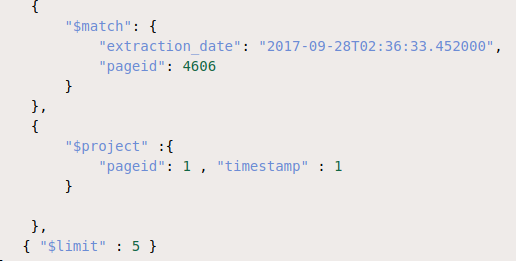
\includegraphics[width=1\textwidth]{figures/query_body_format}
	\caption{Estructura del cuerpo de la petición a la ruta /api/v1/query}
	\label{fig:query_body_format}
\end{figure}

Adicionalmente, la ruta permite especificar la colección de la base de datos a la cual consultar, y de forma opcional,
el formato de fecha de alguna columna en caso de ser necesario.
Un ejemplo, del uso de estos parámetros es el que se muestra en la figura \ref{fig:query_url}, en donde se realiza una consulta de la colección llamada \texttt{revisions}

\begin{figure}[H]
	\centering
		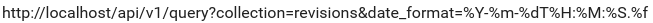
\includegraphics[width=1\textwidth]{figures/query_url}
	\caption{Estructura del cuerpo de la petición a la ruta /api/v1/query}
	\label{fig:query_url}
\end{figure}

Por medio de esta ruta es posible realizar cualquier tipo de consulta sobre la base de datos, y así, obtener métricas
adicionales para su análisis posterior. En la tabla \ref{tab:query} se puede ver mas detalles con respecto a los parámetros.

\begin{longtable}{|l|m{4in}|}

\hline
\multicolumn{2}{|r|}{\textbf{Historia}} \\
\hline
\endfirsthead

\multicolumn{2}{c}%
{{\bfseries \tablename\ \thetable{} -- continuación de la página anterior}} \\
\hline \multicolumn{2}{|r|}{\textbf{Historia}} \\ \hline
\endhead

\textbf{Desarrollador} & Francisco Delgado \\
\hline
\textbf{Nombre} & Endpoint para la consultas directas a la base de datos \\
\hline
\textbf{Sección} & Consulta\\
\hline
\textbf{Descripción} & Parte del API de la solución distribuida donde el endpoint \texttt{/query}
recibe el contenido de la consulta a realizar en formato JSON, a través del cuerpo de la solicitud que se realiza. Dicho cuerpo debe tener un formato adecuado para realizar la consulta en base al módulo Pymongo.
\par Además de esto, existen 2 argumentos opcionales:
\par
\tabitem collection: la colección sobre la cuál se hará la consulta.
 Su valor por defecto es la colección \texttt{revisions}.
\par
\tabitem date\_format: el formato se fecha que será usado en la consulta. 
Su valor por defecto es \texttt{\%Y-\%m-\%dT\%H:\%M:\%S}. 
Donde cada letra excepto la T representa el valor de unidad de tiempo correspondiente en inglés, por ejemplo Y para Año (Year). 
La letra T representa la finalización de la sección de la fecha y el inicio de la sección del tiempo en el formato.

\\
\hline
\textbf{Observaciones} & \\
\hline
\caption{Consultas Directas a la Base de Datos}
\label{tab:query}
\end{longtable}



\subsection{Algoritmo de Revisita}

Una vez el proceso de extracción esta completo,
es necesario mantener una actualización constante de los historiales declaración articulo.
Para ello se hace uso de un algoritmo, al cual llamaremos algoritmo de revisita, que determine, acorde a ciertos coeficientes, si
es necesarios ejecutar una petición de extracción de los historiales de un artículo.
Este algoritmo es ejecutado en segundo plano como una tarea programada, y para ello
se hace uso del programa llamado Cron.
Cron es un planificador de tareas, basado en tiempo, para sistemas operativos basados en Unix, que permite la ejecución de programas o comandos de forma automática en una fecha o frecuencia de tiempo determinado \cite{24}.

El código fuente \ref{code:crontab} muestra el proceso de edición del archivo de configuración previamente mencionado, en donde se hace uso del comando \texttt{crontab -e}
para acceder fácilmente al archivo, y ademas, se muestra el formato aceptado por Cron
para asignar la frecuencia de ejecución.

\begin{minipage}{\linewidth}
\begin{lstlisting}[caption={Edición del archivo de configuración de Cron},breaklines=true,label={code:crontab}]
$ crontab -e
#---------------- Minutos (0 - 59)
|  #------------- Horas (0 - 23)
|  |  #---------- Dia del mes (1 - 31)
|  |  |  #------- Mes (1 - 12)
|  |  |  |  #---- Dia de la semana (0 - 6) (Domingo=0)
|  |  |  |  |
*  *  *  *  *  ejemplo-script.sh
\end{lstlisting}
\end{minipage}

La configuración de Cron para el algoritmo de revisita puede ser apreciado en el código fuente \ref{code:crontab_revisit}, en el cual el comando \texttt{python -m app.cronjobs.revisit} se ejecuta de forma diaria a las 12:00AM.

\begin{minipage}{\linewidth}
\begin{lstlisting}[caption={Edición del archivo de configuración de Cron},breaklines=true,label={code:crontab_revisit}]
$ crontab -e
0 0 * * * python -m app.cronjobs.revisit
\end{lstlisting}
\end{minipage}

El algoritmo de revisita hace uso de un modelo probabilístico que calcula el coeficiente del tiempo revisita de cada artículo wiki de manera independiente haciendo uso de la distribución probabilística exponencial.

El objetivo es buscar un valor esperado de tiempo que mida la distancia entre dos revisiones para ejecutar una revisita de una articulo wiki.
Para ello, se plantea utilizar la fórmula de la esperanza matemática proveniente de la distribución de probabilidad exponencial, la cual es adecuada para estos casos, puesto que la misma estudia la longitud de los intervalos de una variable.

Siendo $x$  una variable aleatoria que sigue una distribución exponencial, la cual mide el intervalo de tiempo transcurrido entre dos revisiones de un artículo de wiki;
y sea $\lambda$ el promedio de revisiones por unidad de tiempo, podemos obtener valor medio o esperanza  matemática de $x$ con la siguiente fórmula:

\begin{gather*}
E(x) = 1 / \lambda
\end{gather*}

Para calcular el promedio de revisiones por unidad de tiempo, se toma una muestra de las revisiones almacenadas en el sistema.
Es necesario que se tome en cuenta que cada artículo wiki tiene una frecuencia de revisiones que la distingue de las demás.
Por ejemplo, para eventos deportivos recurrentes como las olimpiadas o copas mundiales de fútbol, la cantidad de revisiones que se ejercen sobre dichos artículos disminuyen drásticamente una vez culminado el evento, por lo que su frecuencia varía dependiendo de qué intervalos de tiempo se tome en cuenta a la hora de evaluarlos.
Por lo tanto, para poder obtener el valor más adecuado a la frecuencia actual de los artículos, se toma como muestra el mayor número entre: las últimas 20 revisiones del artículo y el más reciente 10\% de la cantidad total de revisiones del artículo.

Una vez vez extraída la muestra, es posible calcular $\lambda$ con la siguiente fórmula:

\begin{gather*}
\lambda = n / (t1 - t0)
\end{gather*}

Siendo $n$ el número de revisiones de la muestra;
$t1$ la fecha de la revisión más reciente en la muestra;
y $t2$ la fecha de la revisión más antigua en la muestra.

Por último, se toma la fecha de la última revisión y se calcula la diferencia entre la fecha actual.
Si dicho valor es mayor a la esperanza matemática $E(x)$, entonces se volverá a visitar el artículo.
A medida que el  se eleve, menor es el intervalo de tiempo entre cada ocurrencia, y por lo tanto, el intervalo de tiempo entre cada revisita del artículo es menor.

Usemos 2 casos de ejemplo:

\begin{itemize}

\item El artículo A tiene 280 revisiones almacenadas en el sistema.

  \begin{enumerate}
  \item Se determina el valor más alto entre 20 y el 10\% de 280.

  \begin{gather*}
  100\% = 280 \text{revisiones}\\
  10\% = x\\
  x = (280 \text{revisiones} \times 10\%) / 100\%\\
  x = 28 \text{revisiones}
  \end{gather*}

  Se toma 28 como el número de la muestra a evaluar.

  Se calcula el intervalo de tiempo entre la primera y la última revisión $(t1 - t0)$ de la muestra de 28 revisiones.
  Asumamos que dicho valor es de 14 días, con el cual podemos calcular $\lambda$ de la siguiente manera:

  \begin{gather*}
  \lambda = n / (t1 - t0)\\
  \lambda = 28 \text{revisiones} / 14 \text{días}\\
  \lambda = 2 \text{revisiones} / \text{día}
  \end{gather*}

  \item Ahora, para calcular el valor de la esperanza:

  \begin{gather*}
  E(x)= 1 / \lambda\\
  E(x)= 1 / (2 \text{revisiones} / \text{día})\\
  E(x)= 0.5 (\text{días} / \text{revisión})
  \end{gather*}

  \item A continuación, podemos convertir la esperanza a otra unidad de tiempo más conveniente, por ejemplo horas, haciendo una conversión básica:

  \begin{gather*}
  E(x)= (0.5 \text{días} / \text{revisión}) * (24\text{horas}/1 \text{día})\\
  E(x)= 0.5*24 \text{horas} / \text{revisión} \\
  E(x) = 12 \text{horas}/ \text{revisión}
  \end{gather*}

  \item Si han pasado más de 12 horas desde la fecha de la última revisión, el artículo será encolado para su extracción.

  \end{enumerate}

\item El artículo B tiene 1350 revisiones almacenadas en el sistema.

  \begin{enumerate}

  \item Se determina el valor más alto entre 20 y el 10\% de 1350.

  \begin{gather*}
  100\% = 1350 \text{revisiones}\\
  10\% = x\\
  x = (1350 \text{revisiones} *10\%) / 100\% \\
  x = 135 \text{revisiones}
  \end{gather*}

  \item Se toma 135 como el número de la muestra a evaluar.

  \item Se calcula el intervalo de tiempo entre la primera y la última revisión $(t1 - t0)$ de la muestra de 135 revisiones.
  Asumamos que dicho valor es de 13 días, con el cual podemos calcular $\lambda$ de la siguiente manera:

  \begin{gather*}
  \lambda = n / (t1 - t0)\\
  \lambda = 135 \text{revisiones} / 13 \text{días} \\
  \lambda = 10.38 \text{revisiones} / \text{día}\\
  \end{gather*}

  \item Ahora, para calcular el valor de la esperanza:

  \begin{gather*}
  E(x)= 1 / \lambda\\
  E(x)= 1/ ( 10.38 \text{revisiones} / \text{día})\\
  E(x)= 0.096 (\text{días} / \text{revisión})
  \end{gather*}

  \item A continuación, podemos convertir la esperanza a otra unidad de tiempo más conveniente, por ejemplo horas, haciendo una conversión básica:

  \begin{gather*}
  E(x) = (0.096 \text{días} / \text{revisión}) * (24\text{horas}/1 \text{día})\\
  E(x) = 0.096*24 \text{horas} / \text{revisión}\\
  E(x) = 2.31 \text{horas}/ \text{revisión}
  \end{gather*}

  \end{enumerate}
\end{itemize}

Con esto, se puede verificar que en intervalos de mayor actividad, el algoritmo de revisita puede mantener un buen rendimiento.

La tabla \ref{tab:revisit}, mostrada a continuación, representa la historia asociada al algoritmo de revisita.

\begin{longtable}{|l|m{4in}|}

\hline
\multicolumn{2}{|r|}{\textbf{Historia}} \\
\hline
\endfirsthead

\multicolumn{2}{c}%
{{\bfseries \tablename\ \thetable{} -- continuación de la página anterior}} \\
\hline \multicolumn{2}{|r|}{\textbf{Historia}} \\ \hline
\endhead

\textbf{Desarrollador} & Marvin Bernal \\
\hline
\textbf{Nombre} & Algoritmo de Revisita \\
\hline
\textbf{Sección} & Extracción \\
\hline
\textbf{Descripción} & Algoritmo para la extracción de nuevas revisiones de los artículos almacenados. Calcula la esperanza matemática de cada artículo en base a la función probabilística exponencial, 
para estimar cuando un artículo tenga una o mas revisiones pendientes no almacenadas en la base de datos. 
\par Para el cálculo de la esperanza se toma el 10\% más reciente de revisiones, 
y el tiempo transcurrido entre estas. 
Con estos datos, se calcula la esperanza y se verifica si el tiempo desde la última revisión es mayor a la misma. En caso positivo, el artículo es encolado para su extracción.
\\
\hline
\textbf{Observaciones} & Se ejecuta en segundo plano por medio de un cronjob diariamente.\\
\hline
\caption{Algoritmo de revisita de revisiones de artículos wiki}
\label{tab:revisit}
\end{longtable}



\subsection{Almacenamiento}

Como fue mencionado en el Capítulo 2, la base de datos utilizada para almacenar las revisiones y artículos wiki es MongoDB.
A través del proceso de extracción se almacenan dos colecciones:
\texttt{revisions}, que representa las revisiones o historial de modificaciones del artículo wiki;
y \texttt{articles}, que se refiere a los artículos de dichas revisiones.
La arquitectura elegida para esta solución contiene la cantidad de elementos mínimos para implementar un cluster de base de datos en MongoDB, y cuenta con: dos sets de réplicas de shards, un set de réplicas para el servidor de configuración, y por último, un servidor de consultas.

La tabla \ref{tab:database} representa la historia asociada al almacenamiento de los datos en MongoDB.

\begin{longtable}{|l|m{4in}|}

\hline
\multicolumn{2}{|r|}{\textbf{Historia}} \\
\hline
\endfirsthead

\multicolumn{2}{c}%
{{\bfseries \tablename\ \thetable{} -- continuación de la página anterior}} \\
\hline \multicolumn{2}{|r|}{\textbf{Historia}} \\ \hline
\endhead

\textbf{Desarrollador} & Francisco Delgado \\
\hline
\textbf{Nombre} & Almacenamiento de Revisiones \\
\hline
\textbf{Sección} & Base de Datos \\
\hline
\textbf{Descripción} & Conjunto de funciones para la conexión, consulta e inserción de
datos en la base de datos (MongoDB). Realizada con el lenguaje
Python y definidas dentro de una clase, se encarga de brindar una
capa de interacción entre MongDB y todas las operaciones de
lectura/escritura de revisiones de un articulo wiki.
\\
\hline
\textbf{Observaciones} & Las operaciones de escritura detectan si la revisión a insertar es
un duplicado por medio del identificador único de la revisión
(revid), y posteriormente procede a actualizar los datos ya existentes con los de la nueva entrada.
\par
Se genera una nueva conexión con la base de datos por cada
operación que se requiera ejecutar en vez de utilizar una o más
conexiones en común para llevar a cabo las tareas.\\
\hline
\caption{Almacenamiento de revisiones de artículos wiki}
\label{tab:database}
\end{longtable}


Las colecciones están distribuidas entre dos fragmentos o shards que contienen un subgrupo de los datos fragmentados en el cluster, y la unión de estos subgrupos conforman la totalidad de los datos almacenados por la aplicación.
Esta separación de los datos puede ser apreciada en la figura \ref{fig:sharded_database}.

\begin{figure}[H]
	\centering
		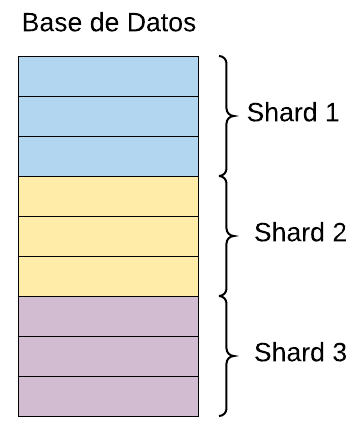
\includegraphics[width=0.4\textwidth]{figures/sharded_database}
	\caption{División de la base de datos en subgrupos}
	\label{fig:sharded_database}
\end{figure}

Cada uno de estos subgrupos está siendo almacenado un servidor físico diferente, garantizando el escalamiento horizontal, tal como lo demuestra la figura \ref{fig:shards_distributed},
Para la creación de estos grupos, el sharding se lleva a cabo a través del Hashed Sharding, de esta manera es
posible alcanzar una distribución homogénea de los datos entre los servidores.

\begin{figure}[H]
	\centering
		
\includegraphics[width=0.5\textwidth]{figures/shards_distributed}
	\caption{Shards de la base de datos distribuidos físicamente}
	\label{fig:shards_distributed}
\end{figure}

Para poder crear un shard es necesario que este pertenezca a un set de réplica de un mínimo de tres miembros,
por lo tanto, por cada shard se tienen tres servidores físicos que permiten la replicación de ese subgrupo de datos, garantizando
así la alta disponibilidad de los mismos.
Para poder fragmentar la base de datos, se necesita de un mínimo de dos shards, por lo que se tiene un total mínimo de 6 servidores
que solo cumplen las labores de fragmentación y replicación.

Para poder coordinar las funciones de estos shards, como la autenticación, almacenamiento de los meta datos y consultas sobre el cluster de shards,
es necesario hacer uso del servicio de un servidor de configuración.
Este servidor, al igual que los shards, debe pertenecer a un grupo de réplicas, sumando tres servidores físicos mas, que ademas,
tienen la capacidad de recuperarse en caso de fallos, y nuevamente, permitir la alta disponibilidad.

Finalmente, se tiene un último servidor de base de datos cuya única labor es la ejecución de operaciones de lectura y escritura sobre la base de datos.
Este servidor es denominado servidor de consultas y no es necesaria su replicación.
Las aplicaciones clientes que deseen realizar alguna consulta sobre la base de datos, realizan sus peticiones únicamente a este servidor.
Así mismo, una vez es recibida la petición de consulta, este se comunica con servidor de configuración para que este le brinde apoyo a la hora de ejecutar las operaciones.
Con este último servidor, el conteo total de servidores de MongoDB para está arquitectura es de diez nodos.

La figura \ref{fig:mongo_cluster}, que se muestra a continuación, demuestra el diagrama de la arquitectura del cluster de base de datos implementado:

\begin{figure}[H]
	\centering
		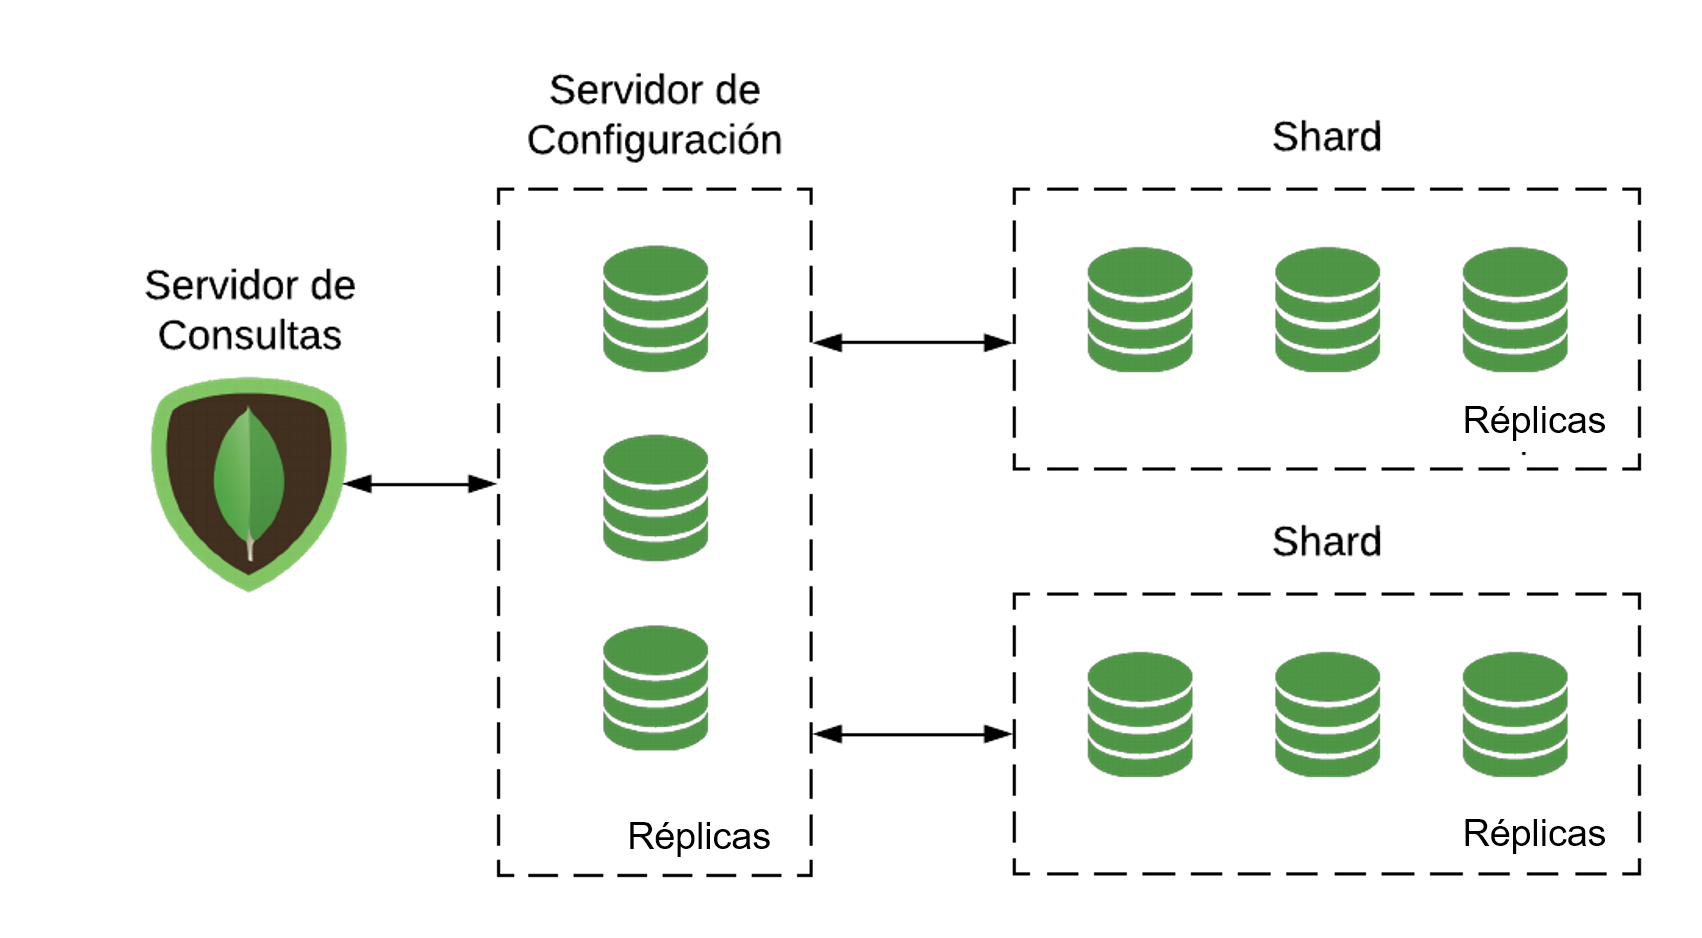
\includegraphics[width=0.9\textwidth]{figures/mongo_cluster}
	\caption{Arquitectura del cluster de base de datos}
	\label{fig:mongo_cluster}
\end{figure}

En tabla \ref{tab:cluster} se puede apreciar la historia asociada a la configuración del cluster de MongoDB.

\begin{longtable}{|l|m{4in}|}

\hline
\multicolumn{2}{|r|}{\textbf{Historia}} \\
\hline
\endfirsthead

\multicolumn{2}{c}%
{{\bfseries \tablename\ \thetable{} -- continuación de la página anterior}} \\
\hline \multicolumn{2}{|r|}{\textbf{Historia}} \\ \hline
\endhead

\textbf{Desarrollador} & Francisco Delgado \\
\hline
\textbf{Nombre} & Configuración de Shards y Réplicas  \\
\hline
\textbf{Sección} & Base de Datos \\
\hline
\textbf{Descripción} & Configuración de los diversos nodos que incluidos dentro del cluster
de la base de datos.
Se configuran dos servidores para la fragmentación de datos por medio de Hashed Sharding.
Cada un de ellos forma parte de un grupo de réplicas, por lo que se hace uso de tres servidores
por nodo de fragmentación.
\par
Se elige un nodo principal por cada grupo de réplica, en este nodo se inicializa la configuración del grupo por medio del comando \verb|rs.initiate()|.
Posteriormente se agregan los dos miembros restantes del grupo usando \verb|rs.add('mongors1n2:27018')| y \verb|rs.add('mongors1n3:27018')|.
Luego, con estos grupos de réplicas ya creados, se generan los shards con el siguiente comando:
\verb|sh.addShard('mongors1/mongors1n1:27018')|. Y, finalmente, se habilita el sharding por medio del comando \verb|sh.enableSharding('wiki_history_extractor')|

Una vez las réplicas y shards, han sido configurados, se genera una réplica extra para el servidor de configuración, el cual ayuda a la coordinación y consulta de los shards.

\\
\hline
\textbf{Observaciones} & Para los grupos de réplicas no fue implementado un algoritmo de selección
de nodo maestro, por lo cual se hace uso del comportamiento por defecto de
MongoDB para elegirlo.\\
\hline
\caption{Configuración del cluster de MongoDB}
\label{tab:cluster}
\end{longtable}


\subsection{Docker}

Para poder poner en funcionamiento esta aplicación distribuida y el cluster de la base de datos, se hace uso de la herramienta Docker.
Docker permite levantar servicios que emulan un servidor físico, los cuales pueden ser conectados en una red para que puedan comunicarse y llevar a cabo todas las tareas de extracción y consultas.

Adicionalmente, permite generar ambientes tanto de producción como de desarrollo, en este caso, se hace uso de la versión \texttt{17.12.0-ce} en conjunto con Docker-Compose para facilitar el levantamiento de los servicios en ambos ambientes.

En la tabla \ref{tab:docker}, que se presenta a continuación, se puede apreciar la historia asociada al uso de docker para el levantamiento de la aplicación.

\begin{longtable}{|l|m{4in}|}

\hline
\multicolumn{2}{|r|}{\textbf{Historia}} \\
\hline
\endfirsthead

\multicolumn{2}{c}%
{{\bfseries \tablename\ \thetable{} -- continuación de la página anterior}} \\
\hline \multicolumn{2}{|r|}{\textbf{Historia}} \\ \hline
\endhead

\textbf{Desarrollador} & Francisco Delgado \\
\hline
\textbf{Nombre} & Automatización de levantamiento de la aplicación \\
\hline
\textbf{Sección} & Configuración de aplicación distribuida \\
\hline
\textbf{Descripción} & Configuración de las imágenes y contenedores de docker para el levantamiento
de la aplicación, distribución de las tareas entre diversos nodos, y levantamiento del cluster de MongoDB.
\\
\hline
\textbf{Observaciones} & La configuración de los contenedores se realiza por medio del archivo \texttt{docker-compose.yml}. Se implementó un archivo por cada ambiente de desarrollo, los cuales son: Digital Ocean, el cual es un servicio de alojamiento web y sirve como ambiente de producción sin la inclusion de las replicas de mongo;
Desarrollo, para es el ambiente para desarrollo continuo de la aplicación;
y por ultimo, Replica, el cual define la configuración completa del cluster de MongoDB y sirve como ambiente de producción \\
\hline
\caption{Configuración del levantamiento de la aplicación por medio de Docker}
\label{tab:docker}
\end{longtable}


En primera instancia se genera una imagen para la aplicación flask, los trabajadores de Celery y el resto de los servicios.
El nombre de las imágenes está definido bajo el siguiente formato: \texttt{nombre:version}, y pueden ser generadas por medio de un archivo llamado Dockerfile, cuyo contenido puede ser apreciado a continuación:

\begin{minipage}{\linewidth}
\begin{lstlisting}[language=docker,caption={Contenido del archivo Dockerfile para la imagen del API},breaklines=true,label={code:dockerfile}]
# Dockerfile
FROM python:2.7-alpine

RUN mkdir /app
WORKDIR /app

COPY requirements.txt requirements.txt
RUN pip install -r requirements.txt

COPY . .

CMD python manage.py runserver --host 0.0.0.0 --port=80
\end{lstlisting}
\end{minipage}

Para los servicios de Nginx, RabbitMQ y MongoDB se hace uso de imágenes provenientes del repositorio oficial llamado Docker Hub,
las imágenes utilizadas son las siguientes: \texttt{rabbitmq:3.6.11}, \texttt{mongo:3.6.2} y \texttt{nginx:1.13.3}.

La configuración de los contenedores se realiza a través del archivo \texttt{docker-compose.yml}, en el cual se especifican
las imágenes a utilizar por cada servicio, variables de entorno, nombre de la red, entre otros.

Las imágenes de RabbitMQ y MongoDB tienen la característica que permite utilizar variables de entorno para establecer el usuario y clave de acceso sin ningún tipo de configuración manual por parte del desarrollador,
por lo tanto, las credenciales usadas para ambos servicios son agregadas en el archivo \texttt{docker-compose.yml} para restringir su acceso.
Por ejemplo, para RabbitMQ las credenciales son las siguientes: \verb|RABBITMQ_DEFAULT_USER=wiki| y \verb|RABBITMQ_DEFAULT_PASS=wiki123|.
Adicionalmente, se establecieron una serie reglas adicionales, como por ejemplo,
declaración de volúmenes para mantener la persistencia de datos y
la exposición de los puertos de RabbitMQ, MongoDB y Nginx;
lo cual permite a las aplicaciones externas acceder a estos servicios, y en el caso de Nginx, permite que otras aplicaciones puedan ejecutar peticiones al API.

Parte de la configuración de los servicios y contendedores de Docker puede ser apreciada a continuación:

\begin{minipage}{\linewidth}
\begin{lstlisting}[language=docker-compose-2,caption={Declaración de servicios con Docker Compose},breaklines=true,label={code:dockercompose}]
version: '3'

services:

    rabbit:
        image: rabbitmq:3.6.11
        restart: always
        hostname: rabbit
        environment:
            - RABBITMQ_DEFAULT_USER=wiki
            - RABBITMQ_DEFAULT_PASS=wiki123
        ports:
            - "5673:5672"
        networks:
            - wiki_network
        volumes:
            - 'wiki_rabbit:/data'
\end{lstlisting}
\end{minipage}
